\documentclass[10pt,a4paper]{article}
\usepackage[utf8]{inputenc}
\usepackage{graphicx}
\def\Pr{\mathop{\rm Pr}}
\usepackage[landscape,margin=1cm]{geometry}
\usepackage[english]{babel}
\usepackage{tikz}
\usetikzlibrary{arrows,snakes,backgrounds,shapes.geometric}
\title{Probability and Statistical Inference}
\author{John S Butler}
%\date{July 2019}
\input{cheatsheet-template.tex}



%--------------------------------------------------------------------------------
\begin{document}
\small
\begin{multicols}{3}

%\maketitle
%\thispagestyle{empty}
\scriptsize
%\tableofcontents


%\section{Data Type}
\section*{Introduction to Maths, Flowcharts, and Pseudocode - Algorithms  (MATH1812)\footnote{\href{https://sites.google.com/dit.ie/math1812/home}{Course Website: https://sites.google.com/dit.ie/math1812/home}}}
%$\subsection*{Cheat Sheet}
\subsubsection*{\href{johnsbutler.netlify.com}{John S Butler} (TU Dublin) }
\begin{textbox}{Mathematics - Single Loop}

\begin{subbox}{subbox}{Example 1}
The mathematical expression
\[ \sum_{i=0}^{6} 3i, \]
can be expanded as,
\[ \sum_{i=0}^{6} 3i=3(0)+3(1)+3(2)+3(3)+3(4)+3(5)+3(6), \]
or can be written in tabular form:\\
\begin{tabular}{ c| c c c c c c c}
 $i$&$0$ & $1$ & $2$&$3$ & $4$ & $5$ & $6$\\ \hline
 $3i$&$3(0)$ & $3(1)$ & $3(2)$&$3(3)$ & $3(4)$ & $3(5)$ & $3(6)$
\end{tabular}
where the bottom row is summed giving,
\[ \sum_{i=0}^{6} 3i=63.\]
\end{subbox}

\begin{subbox}{subbox}{Example 2}
The mathematical expression
\[ 10+\sum_{j=-3}^{2} (2+\frac{j}{2}), \]
can be expanded as,
\begin{multline*}
10+\sum_{j=-3}^{2} (2+\frac{j}{2})=10+(2+\frac{-3}{2})+(2+\frac{-2}{2})+(2+\frac{-1}{2})\\+(2+\frac{0}{2})+(2+\frac{1}{2})+(2+\frac{2}{2}),
\end{multline*}
\[ 10+\sum_{j=-3}^{2} (2+\frac{j}{2})=20.5.\]
\end{subbox}

\end{textbox}

\columnbreak

\begin{textbox}{Flowchart  - Single Loop}
\begin{subbox}{subbox}{Example 1}
\begin{center}
    
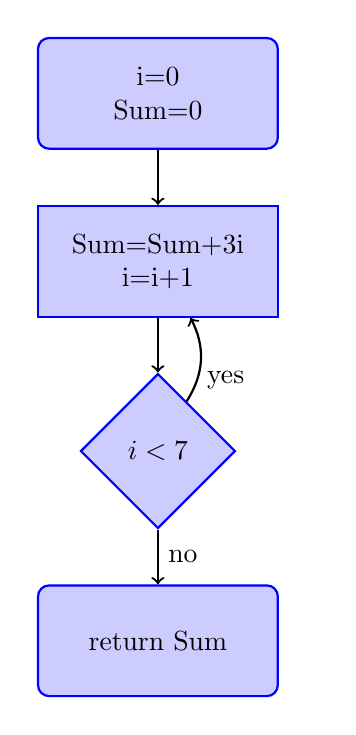
\begin{tikzpicture}[auto]
\tikzstyle{decision} = [diamond, draw=blue, thick, fill=blue!20,
text width=4.5em, text badly centered, inner sep=1pt]

\tikzstyle{block} = [rectangle, draw=blue, thick, fill=blue!20,
text width=8em, text centered, rounded corners, minimum height=4em]
\tikzstyle{block_op} = [rectangle, draw=blue, thick, fill=blue!20,
text width=8em, text centered, minimum height=4em]
\tikzstyle{line} = [draw, thick,->];
\tikzstyle{cloud} = [draw=red, thick, ellipse,fill=red!20, minimum height=2em];
\matrix [column sep=5mm,row sep=7mm]
{
% row 1
 \node [block] (init) {i=0 \\ Sum=0}; & \\
% row 2
\node [block_op] (identify) {Sum=Sum+3i\\
i=i+1}; & ;\\
% row 4
\node [decision] (decide) {$i<7$}; & \\
% row 5
\node [block] (stop) {return Sum}; & \\
};
\tikzstyle{every path}=[line]
\path (init) -- (identify);
\path (identify) -- (decide);
\path (decide)  edge [bend right] node[near start,right] {yes}  (identify);
\path (decide) -- node [midway] {no} (stop);

\end{tikzpicture}

\end{center}
\end{subbox}

\begin{subbox}{subbox}{Example 2}
\begin{center}
    
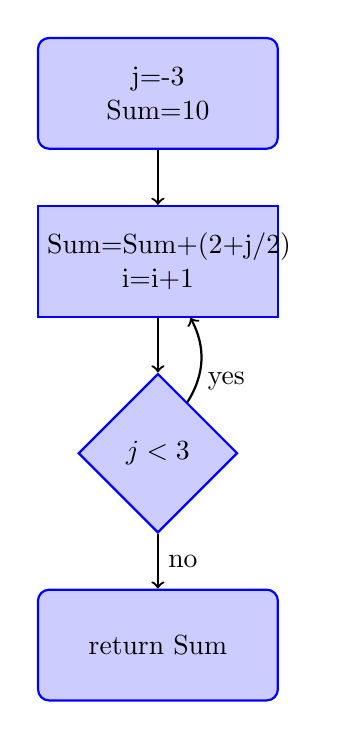
\begin{tikzpicture}[auto]
\tikzstyle{decision} = [diamond, draw=blue, thick, fill=blue!20,
text width=4.5em, text badly centered, inner sep=1pt]

\tikzstyle{block} = [rectangle, draw=blue, thick, fill=blue!20,
text width=8em, text centered, rounded corners, minimum height=4em]
\tikzstyle{block_op} = [rectangle, draw=blue, thick, fill=blue!20,
text width=8em, text centered, minimum height=4em]
\tikzstyle{line} = [draw, thick,->];
\tikzstyle{cloud} = [draw=red, thick, ellipse,fill=red!20, minimum height=2em];
\matrix [column sep=5mm,row sep=7mm]
{
% row 1
 \node [block] (init) {j=-3 \\ Sum=10}; & \\
% row 2
\node [block_op] (identify) {Sum=Sum+(2+j/2)\\
i=i+1}; & ;\\
% row 4
\node [decision] (decide) {$j<3$}; & \\
% row 5
\node [block] (stop) {return Sum}; & \\
};
\tikzstyle{every path}=[line]
\path (init) -- (identify);
\path (identify) -- (decide);
\path (decide)  edge [bend right] node[near start,right] {yes}  (identify);
\path (decide) -- node [midway] {no} (stop);
\end{tikzpicture}
\end{center}
\end{subbox}
\end{textbox}
%%% FLOW CHART
\begin{textbox}{Pseudocode - Single Loop}
\begin{subbox}{subbox}{Example 1}
\begin{codebox}{r}{Python Pseudocode}

# Setting up the initial Sum value
Sum=0

# For loop from 0 to 6 with steps of 1
for i in range(0,7):
    Sum=Sum+3*i
    
    
print(Sum)



\end{codebox}
The line by line output of the code for Example 1 is:
\begin{center}
\begin{tabular}{ c| c| c }
 Loop count &i & Sum \\ \hline
 0&0 & 0  \\
 1&1 & 3  \\
 2&2 & 9  \\
 3&3 & 18  \\
 4&4 & 30  \\
 5&5 & 45 \\
 6&6 & 63
\end{tabular}
\end{center}
\end{subbox}
\vspace{5mm}\\

\begin{subbox}{subbox}{Example 2}
\begin{codebox}{r}{Python Pseudocode}
# Setting up the initial Sum value as 10
Sum=10

# For loop from -3 to 2 with steps of 1
for j in range(-3,3):
    Sum=Sum+(2+j/2)

return Sum
\end{codebox}
The line by line output of the code for Example 2 is:
\begin{center}
\begin{tabular}{ c| c| c }
 Loop count &j & Sum \\ \hline
 0&-3 & 10.5  \\
 1&-2 & 11.5  \\
 2&-1 & 13  \\
 3&0 & 15.0  \\
 4&1 & 17.5  \\
 5&2 & 20.5 
\end{tabular}
\end{center}
\end{subbox}
\end{textbox}
%%%% EXAMPLE 3
\begin{textbox}{Mathematics - Sequential Loops}

\begin{subbox}{subbox}{Example 3}
The mathematical expression

\[ -3+\sum_{i=0}^{4} -2i+\sum_{j=-10}^{-6} (j+1)^2, \]
can be expanded as,
\begin{multline*}
-3+\sum_{i=0}^{4} -2i+\sum_{j=-10}^{-6} (j+1)^2=-3+\\-2(0)+-2(1)+-2(2)+-2(3)+-2(4)+\\
(-10+1)^2+(-9+1)^2+(-8+1)^2+(-7+1)^2+(-6+1)^2,
\end{multline*}
written in tabular form:\\
\begin{tabular}{ c| c c c c c }
 $i$&$0$ & $1$ & $2$&$3$ & $4$  \\ \hline
 $-2i$&$-2(0)$ & $-2(1)$ & $-2(2)$&$-2(3)$ & $-2(4)$ 
\end{tabular}
where the bottom row is summed giving,
\[ \sum_{i=0}^{4} -2i=-20,\]

the second summation is written in tabular form,\\
\begin{tabular}{ c| c c c c c c }
 $j$&$-10$ & $-9$ & $-8$&$-7$ & $-6$ \\ \hline
 $ (j+1)^2$&$ (-9)^2$ & $(-8)^2$ & $(-7)^2$&$(-6)^2$ & $(-5)^2$
\end{tabular}
summing the bottom row gives,
\[ \sum_{j=-10}^{-6} (j+1)^2=255,\]
bringing this all together,
\[ -3+\sum_{i=0}^{4} -2i+\sum_{j=-10}^{-6} (j+1)^2=-3-20+255=232. \]

\end{subbox}

\end{textbox}

\columnbreak

\begin{textbox}{Flowchart - Sequential Loops}
\begin{subbox}{subbox}{Example 3}
\begin{center}
    
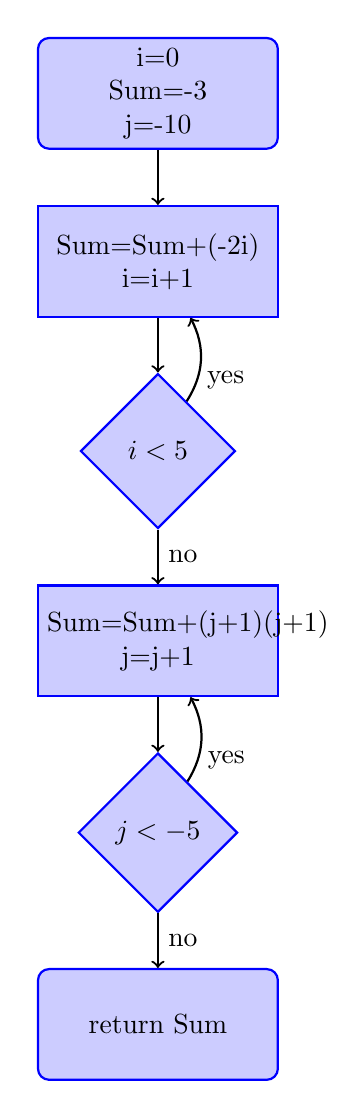
\begin{tikzpicture}[auto]
\tikzstyle{decision} = [diamond, draw=blue, thick, fill=blue!20,
text width=4.5em, text badly centered, inner sep=1pt]

\tikzstyle{block} = [rectangle, draw=blue, thick, fill=blue!20,
text width=8em, text centered, rounded corners, minimum height=4em]
\tikzstyle{block_op} = [rectangle, draw=blue, thick, fill=blue!20,
text width=8em, text centered, minimum height=4em]
\tikzstyle{line} = [draw, thick,->];
\tikzstyle{cloud} = [draw=red, thick, ellipse,fill=red!20, minimum height=2em];
\matrix [column sep=5mm,row sep=7mm]
{
% row 1
 \node [block] (init) {i=0 \\ Sum=-3\\j=-10}; & \\
% row 2
\node [block_op] (identify) {Sum=Sum+(-2i)\\
i=i+1}; & ;\\
% row 4
\node [decision] (decide) {$i<5$}; & \\
% row 5
\node [block_op] (identify2) {Sum=Sum+(j+1)(j+1)\\
j=j+1}; & ;\\
\node [decision] (decide2) {$j<-5$}; & \\
\node [block] (stop) {return Sum}; & \\
};
\tikzstyle{every path}=[line]
\path (init) -- (identify);
\path (identify) -- (decide);
\path (decide)  edge [bend right] node[near start,right] {yes}  (identify);
\path (decide) -- node [midway] {no} (identify2);
\path (identify2) -- (decide2);
\path (decide2)  edge [bend right] node[near start,right] {yes}  (identify2);
\path (decide2) -- node [midway] {no} (stop);
\end{tikzpicture}

\end{center}
\end{subbox}

\end{textbox}


%%% FLOW CHART
\begin{textbox}{Pseudocode - Sequential Loops}
\begin{subbox}{subbox}{Example 3}
\begin{codebox}{r}{Python Pseudocode}
# Setting up the initial Sum value
Sum=-3

for i in range(0,5):
    Sum=Sum+(-2*i)
    print(Sum)
    print(i)
    
for j in range(-10,-5):
    Sum=Sum+(j+1)*(j+1)
    print(Sum)
    print(j)
    
Sum
\end{codebox}
The line by line output of the code for Example 3 is:
\begin{center}
\begin{tabular}{ c| c| c }
 Count &i & Sum \\ \hline
 0 & & -3  \\
 \hline
  &i & -2i \\ \hline
 1&0 & -3  \\
 2&1 & -5  \\
 3&2 & -9  \\
 4&3 & -15  \\
 5&4 & -23  \\
 \hline
   &j & (j+1)(j+1) \\ \hline
 6&-10 & 58  \\
 7&-9 & 122  \\
 8&-8 & 171  \\
 9&-7 & 207  \\
 10&-6 & 232  
\end{tabular}
\end{center}
\end{subbox}
\end{textbox}
%%%% EXAMPLE 3
\begin{textbox}{Mathematics - Double Loop}

\begin{subbox}{subbox}{Example 4 - Double Loop}
The mathematical expression

\[ \sum_{i=0}^{3}\sum_{j=0}^{3} (i^2+3j), \]
can be expanded as,
\begin{multline*}
\sum_{i=0}^{3}\sum_{j=0}^{2} (3j+i^2)=(0^2+3\times 0)+(1^2+3\times 0)+\\
(2^2+3\times 0)+(3^2+3\times 0)+\\
(0^2+3\times 1)+(1^2+3\times 1)+\\
(2^2+3\times 1)+(3^2+3\times 1)+\\
(0^2+3\times 2)+(1^2+3\times 2)+\\
(2^2+3\times 2)+(3^2+3\times 2)\\
\end{multline*}

\end{subbox}

\end{textbox}

\columnbreak

\begin{textbox}{Flowchart - Double Loop}
\begin{subbox}{subbox}{Example 4 - Double Loop}
\begin{center}
    
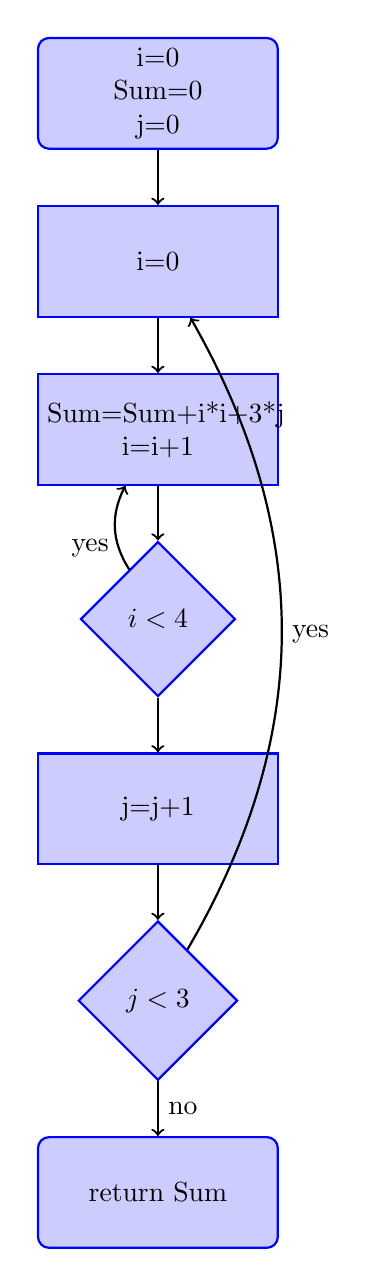
\begin{tikzpicture}[auto]
\tikzstyle{decision} = [diamond, draw=blue, thick, fill=blue!20,
text width=4.5em, text badly centered, inner sep=1pt]

\tikzstyle{block} = [rectangle, draw=blue, thick, fill=blue!20,
text width=8em, text centered, rounded corners, minimum height=4em]
\tikzstyle{block_op} = [rectangle, draw=blue, thick, fill=blue!20,
text width=8em, text centered, minimum height=4em]
\tikzstyle{line} = [draw, thick,->];
\tikzstyle{cloud} = [draw=red, thick, ellipse,fill=red!20, minimum height=2em];
\matrix [column sep=5mm,row sep=7mm]
{
% row 1
 \node [block] (init) {i=0 \\ Sum=0\\j=0}; & \\
% row 2
\node [block_op] (identify) {i=0}; & ;\\
% row 4
\node [block_op] (identify2) {Sum=Sum+i*i+3*j\\
i=i+1}; & ;\\
\node [decision] (decide) {$i<4$}; & \\
% row 5
\node [block_op] (identify3) {
j=j+1}; & ;\\
\node [decision] (decide2) {$j<3$}; & \\
\node [block] (stop) {return Sum}; & \\
};
\tikzstyle{every path}=[line]
\path (init) -- (identify);
\path (identify) -- (identify2);
%\path (identify) -- (decide);
%\path (decide)  edge [bend right] node[near start,right] {yes}  (identify);
%\path (decide) -- node [midway] {no} (identify2);
\path (identify2) -- (decide);
\path (decide) -- (identify3);

\path (identify3) -- (decide2);
%\path (decide2) -- (stop);

\path (decide2)  edge [bend right] node[right] {yes}  (identify);

\path (decide)  edge [bend left] node[near start,left] {yes}  (identify2);

\path (decide2) -- node [midway] {no} (stop);

\end{tikzpicture}

\end{center}
\end{subbox}

\end{textbox}
%%% FLOW CHART
\begin{textbox}{Pseudocode -- Double Loop}
\begin{subbox}{subbox}{Example 4 - Double Loop}
\begin{codebox}{r}{Python Pseudocode}
# Setting up the initial Sum value
Sum=0

for i in range(0,4):
    for j in range(0,3):
        Sum=Sum+i*i+3*j
print(Sum)

\end{codebox}
The line by line output of the code for Example 3 is:
\begin{center}
\begin{tabular}{ c| c| c |c}
 Count &i &j & Sum \\ \hline
 0 & &  & 0  \\
 \hline
  & &  & $Sum=Sum+i^2+3*j$  \\
 \hline
 1&0&0 & $0+0^2+3*0 $ \\
 2&1&0 & $0+1^2+3*0 $  \\
 3&2&0 & $1+2^2+3*0 $  \\
 4&3&0 & $5+3^2+3*0 $  \\
 5&0&1 & $14+0^2+3*1 $ \\
 6&1&1 & $17+1^2+3*1 $  \\
 7&2&1 & $21+2^2+3*1 $  \\
 8&3&1& $26+3^2+3*1 $  \\
 9&0&2 & $36+0^2+3*2 $ \\
 10&1&2 & $42+1^2+3*2 $  \\
 11&2&2 & $49+2^2+3*2 $  \\
 12&3&2& $59+3^2+3*2 $  \\
 \hline
 & & & $73 $  \\
\end{tabular}
\end{center}
\end{subbox}
\end{textbox}



%%% FLOW CHART
\end{multicols}

\newpage
\section*{Quick-Find}
\begin{multicols}{2}
\begin{textbox}{Pseudocode - Quick Find}
\begin{codebox}{r}{Python Pseudocode}

def Union(p,q,ID):
	pID=ID[p]
	qID=ID[q]

	if(pID==qID)
		return Connected

	 for i in range(0,10): 
		if ID[i]==pID:
			ID[i]=qID
	count=count-1	
    return ID
\end{codebox}
\end{textbox}
\begin{textbox}{Flowchart }
\begin{subbox}{subbox}{Quick Find - Connecting}
\begin{center}
    
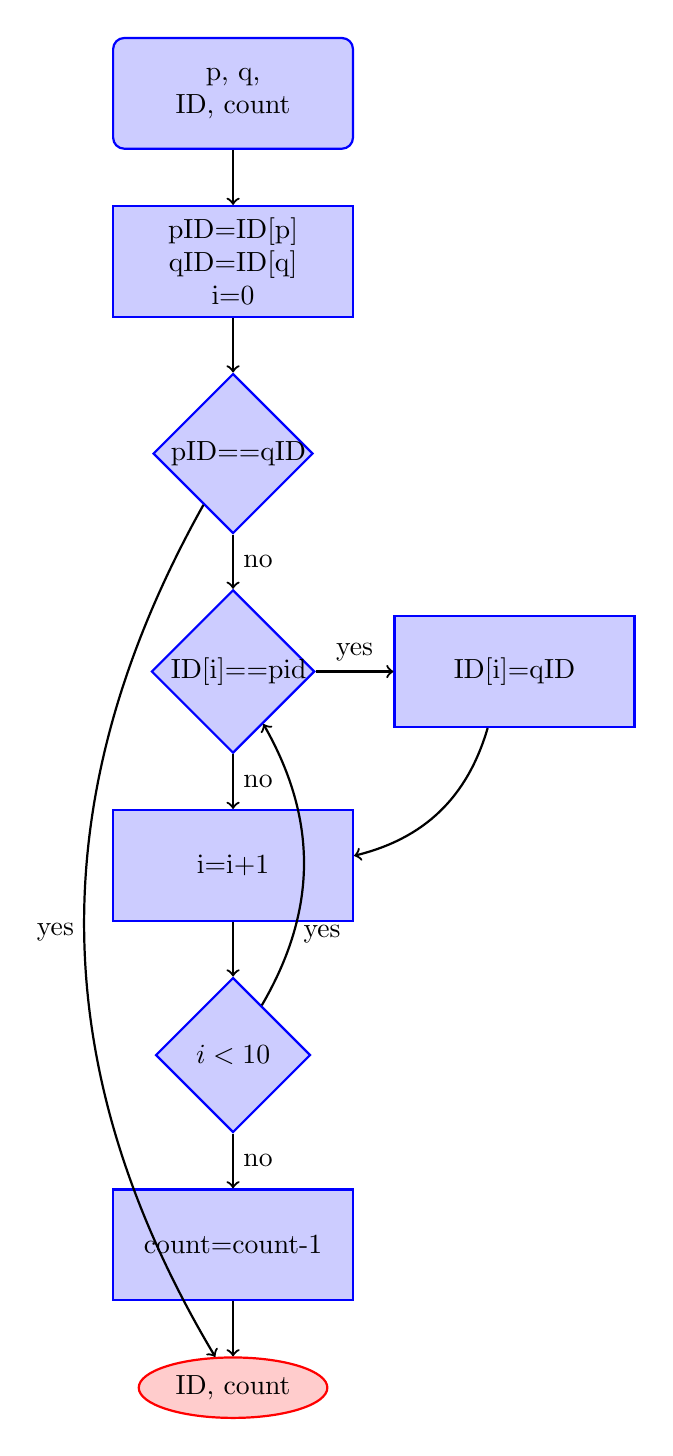
\begin{tikzpicture}[auto]
\tikzstyle{decision} = [diamond, draw=blue, thick, fill=blue!20,
text width=4.5em, text badly centered, inner sep=1pt]

\tikzstyle{block} = [rectangle, draw=blue, thick, fill=blue!20,
text width=8em, text centered, rounded corners, minimum height=4em]
\tikzstyle{block_op} = [rectangle, draw=blue, thick, fill=blue!20,
text width=8em, text centered, minimum height=4em]
\tikzstyle{line} = [draw, thick,->];
\tikzstyle{cloud} = [draw=red, thick, ellipse,fill=red!20, minimum height=2em];
\matrix [column sep=5mm,row sep=7mm]
{
% row 1
 \node [block] (init) {p, q, \\ID, count}; & \\
% row 2
\node [block_op] (identify) {	pID=ID[p]\\
	qID=ID[q]\\ i=0
}; & ;\\
\node [decision] (connect) {pID==qID}; & \\
% row 4

\node [decision] (connect2) {ID[i]==pid}; & \node [block_op] (identify3) {
ID[i]=qID};\\

\node [block_op] (identify2) {i=i+1}; & ;\\
\node [decision] (decide) {$i<10$}; & \\
\node [block_op] (identify4) {count=count-1}; & \\
% row 5
\node [cloud] (stop) {ID, count}; & \\
};
\tikzstyle{every path}=[line]
\path (init) -- (identify);
\path (identify) -- (connect);
\path (connect) -- node [midway]{no}(connect2);
\path (connect2) -- node [midway]{no}(identify2);
\path (connect2) -- node [midway]{yes}(identify3);
\path (identify3) edge [bend left]  (identify2);
\path (connect) edge [bend right] node[left] {yes} (stop);
\path (identify2) -- (decide);
\path (decide)  edge [bend right] node[near start, right] {yes}  (connect2);
\path (decide) -- node [midway] {no} (identify4);
\path (identify4) -- (stop);
\end{tikzpicture}
\end{center}
\end{subbox}
\end{textbox}
%%% Pesudocode
\newpage
%\section*{Quick Union}
\begin{textbox}{Pseudocode -  Quick Union}
\begin{codebox}{r}{Python Pseudocode Find Root}

def root(p, q, ID):
    while (p!=ID[p]):
	    p=ID[p]

    return p 


\end{codebox}
\begin{codebox}{r}{Python Pseudocode Connect}

def Union(p,q,ID,count):
	root_pID=root(p,ID)
	root_qID=root(q,ID)

	if(root_pID==root_qID):
		ID=ID
	else
    	ID[root_pID]=root_qID
    	count=count-1
	return ID


\end{codebox}
\end{textbox}
%%% FLOW CHART
\begin{textbox}{Flowchart Quick Union }
\begin{subbox}{subbox}{Flow Chart Find Root}
\begin{center}
    
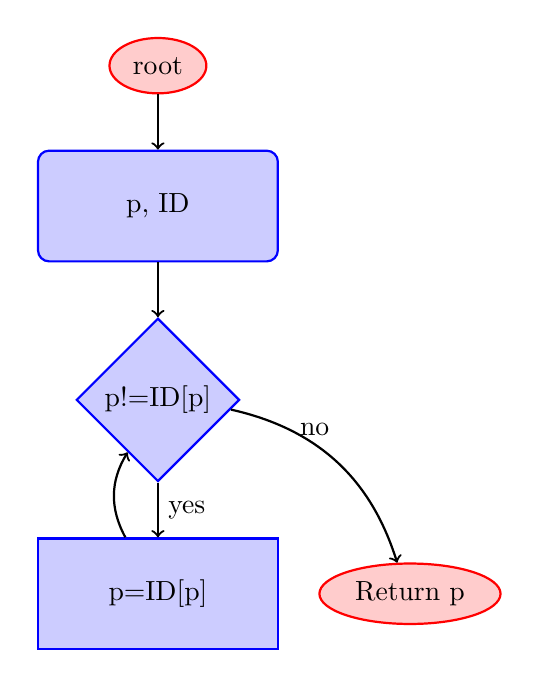
\begin{tikzpicture}[auto]
\tikzstyle{decision} = [diamond, draw=blue, thick, fill=blue!20,
text width=4.5em, text badly centered, inner sep=1pt]

\tikzstyle{block} = [rectangle, draw=blue, thick, fill=blue!20,
text width=8em, text centered, rounded corners, minimum height=4em]
\tikzstyle{block_op} = [rectangle, draw=blue, thick, fill=blue!20,
text width=8em, text centered, minimum height=4em]
\tikzstyle{line} = [draw, thick,->];
\tikzstyle{cloud} = [draw=red, thick, ellipse,fill=red!20, minimum height=2em];
\matrix [column sep=5mm,row sep=7mm]
{
% row 1
\node [cloud] (start) {root};  &;\\
\node [block] (identify) {p, ID
}; & ;\\
\node [decision] (connect) {p!=ID[p]}; & \\

\node [block_op] (identify2) {	p=ID[p]
}; & \node [cloud] (stop) {Return p};\\
};
\tikzstyle{every path}=[line]
\path (start) -- (identify);
\path (identify) -- (connect);
\path (connect) -- node [midway]{yes}(identify2);
\path (connect)edge[bend left] node[near start, right]{no}(stop);
\path (identify2)edge[bend left] (connect);
\end{tikzpicture}

\end{center}
\end{subbox}
\begin{subbox}{subbox}{Flow Chart Connect Nodes}
\begin{center}
    
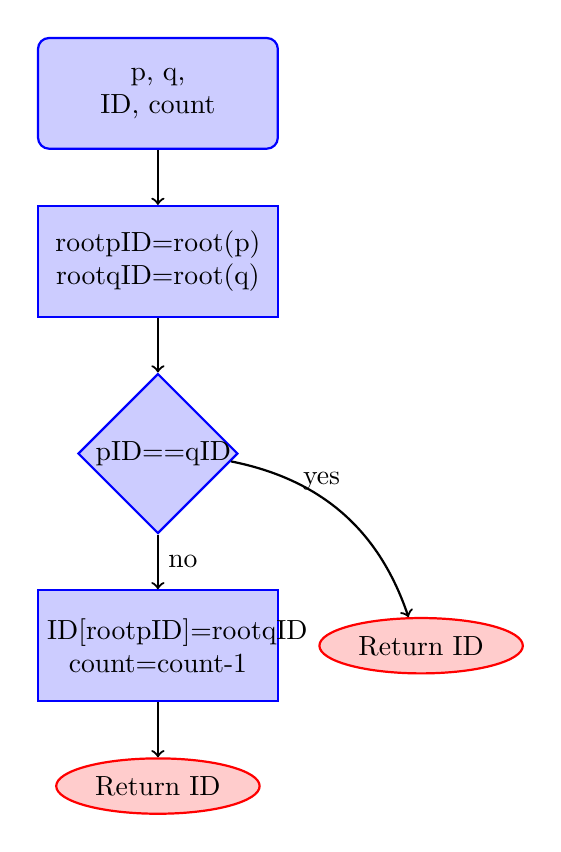
\begin{tikzpicture}[auto]
\tikzstyle{decision} = [diamond, draw=blue, thick, fill=blue!20,
text width=4.5em, text badly centered, inner sep=1pt]

\tikzstyle{block} = [rectangle, draw=blue, thick, fill=blue!20,
text width=8em, text centered, rounded corners, minimum height=4em]
\tikzstyle{block_op} = [rectangle, draw=blue, thick, fill=blue!20,
text width=8em, text centered, minimum height=4em]
\tikzstyle{line} = [draw, thick,->];
\tikzstyle{cloud} = [draw=red, thick, ellipse,fill=red!20, minimum height=2em];
\matrix [column sep=5mm,row sep=7mm]
{
\node [block] (identify) {p, q,\\ ID, count
}; & ;\\
% row 1
\node [block_op] (init) {	rootpID=root(p)\\
rootqID=root(q)
}; & ;\\
\node [decision] (connect) {pID==qID}; & \\
% row 4
\node [block_op] (stopN) {ID[rootpID]=rootqID\\ count=count-1 };&\node [cloud] (stopY) {Return ID};  \\
 \node [cloud] (stop) {Return ID };&;  \\
% row 4
};
\tikzstyle{every path}=[line]
\path (identify) -- (init);
\path (init) -- (connect);
\path (connect)-- node [midway]{no} (stopN);
\path (connect) edge[bend left] node[near start, right]{yes} (stopY);
\path (stopN) -- (stop);
\end{tikzpicture}
\end{center}
\end{subbox}
\end{textbox}

\end{multicols}
\end{document}
